% Template created by Adrienne Traxler (adrienne.traxler@wright.edu)
% Last modified: 3/22/17: Add clarifying note about why the template has too much space around its section headers.
% 
% Changelog
% 3/14/17: add 2-column figure example, tweak text to align with Word sample file, add hyperref for links/cross-references
% 6/21/16: 	Fix old PACS option and superscript affiliations.
% 5/5/16: 	Update sample table to use the REVTEX ruledtabular environment for auto-sizing;
%   		switch to using pra option until the prstper style is fixed (who knows when).
% 5/10/16: Swap suggested department/institution ordering in \affiliation lines.
% 5/12/16: Remove PACS line (deprecated).
% 6/21/16:	Switch to noshowpacs and add superscriptaddress in documentclass options.
% 
% This is my best effort to follow the Physical Review style guide plus specific changes 
% required for PERC (mostly, omitting article titles in references). This version compiles 
% with pdfLaTeX alone; using a proper .bib file changes the bibliography part at the end 
% and would require running BibTex as well.
%
% Finally, there's extra padding around section headers if you compile the bare template. 
% I believe that's because LaTeX stretches its white space to keep the floats (tables and 
% figures) near their input locations. The excess spacing goes away when a normal amount 
% of body text is filled in.

% Big list of reference documentation is here: http://journals.aps.org/revtex, 
%  see especially the APS Author Guide PDF link.

% Notes on the revtex4-1 documentclass options used: 
%  reprint does the double-column, publication ready appearance
%  prstper style formats reference numbers incorrectly, fast fix is to use pra instead.
%  Add longbibliography option to show article titles (and see note in bibliography)

%\documentclass[english,aps,prstper,reprint,showpacs]{revtex4-1}   % This version should work (prstper option), but actually formats reference numbers incorrectly.
\documentclass[english,aps,pra,reprint,noshowpacs,superscriptaddress]{revtex4-1}   
% Using pra instead of prstper gives correct square-bracket (not superscript) reference formatting
\usepackage[T1]{fontenc}	% should generally be included for better accented-word behavior
\usepackage[latin9]{inputenc}	% should generally be included for better accent behavior
\usepackage{geometry}		% for controlling page margins
\geometry{verbose,tmargin=1in,bmargin=1in,lmargin=0.75in,rmargin=0.75in}	% define margins
\usepackage{graphicx}
\usepackage[above,below]{placeins}	% allows use of \FloatBar­rier command to force section barriers
\usepackage{times}
% Next three lines are optional, use the hyperref package to make URLs and reference links live.
\usepackage{hyperref}  
\hypersetup{colorlinks=true,urlcolor=blue,citecolor=blue,linkcolor=blue}   
\urlstyle{same}
\pagestyle{empty}			% page numbers added later, when compiling the whole proceedings
\begin{document}

\title{Paradigms in Physics 2.0}
\author{David Roundy}
\author{Liz Gire}
\author{Ethan Minot}
\author{Emily van Zee}
\affiliation{Department of Physics, Oregon State University, Corvallis, Oregon, 97331}
\author{Tevian Dray}
\affiliation{Department of Mathematics, Oregon State University, Corvallis, Oregon, 97331}
\author{Corinne A. Manogue}
\affiliation{Department of Physics, Oregon State University, Corvallis, Oregon, 97331}

%\keywords{}

\begin{abstract}
In 2016, the Department of Physics at Oregon State University began a
process to revise our Paradigms in Physics curriculum for physics
majors.  This poster will describe both the process by which our
department achieved consensus on this curricular change, and the
resulting curriculum.  The Paradigms 2.0 committee begain with a
survey of students and faculty, followed by individual interviews with
the faculty teaching each existing course.  As we developed a plan to
address student- and faculty-identified challenges in the curriculum,
we met with each faculty member individually to explain and refine our
proposal, which was unanimously approved by the faculty.  Major
changes include elimination or major changes to several courses (math
methods, computational physics, modern physics, electronics, and
classical mechanics), including the introduction of two sophomore-year
courses designed specifically to help prepare students to for their
upper-division courses.
\end{abstract}

\maketitle

\section{Introduction}
The Paradigms in Physics program

\subsection{Background}
\emph{What is the Paradigms now?}
\subsection{History of the Paradigms}
\emph{How did we get here?~\cite{manogue2001paradigms}}
\subsection{Motivation for the change}
\paragraph{Curricular changes}
There were a number of factors that motivated us to embark on the
Paradigms~2.0 process.  The original Paradigms in Physics curricular
reform from 200? was showing its age.  In the intervening years we had
made a large number of modifications, such as reordering Paradigms,
introducing one new Paradigm, and introducing and changing
computational physics courses.  However, there were other changes
needed that could not be separated from an examination of the
curriculum as a whole.  Most notable were discussions of the
requirements for computational physics, the amount of required
electronics credits, and the role of our modern physics course.  These
persistent issues were not easily addressed without addressing the
physics major curriculum as a whole.

\paragraph{New faculty}
At this stage, (XX) of our faculty was not present during the orignal
Paradigms effort.  Many of the newer faculty have only a superficial
undertanding of our course structure.  This poses a challenge when
these professors teach courses that are closely intertwined with one
another.

\section{Paradigms 2.0 process}
\emph{How did we do it?}

%\newcommand\mathcourse[2]{\emph{#1 (#2)}}
\newcommand\mathcourse[2]{\emph{#1}}
\newcommand\noted[2]{\textbf{#1} (#2)}
\newcommand\paradigm[1]{{\sc #1} (3)}
\newcommand\capstone[1]{#1 (3)}
\newcommand\onecredit[1]{#1 (1)}
\newcommand\threecredit[1]{#1 (3)}
\newcommand\fourcredit[1]{#1 (4)}

\begin{table*}[htbp]
\caption{Hypothetical student schedule for a student entering without
  calculus.  Students with AP Calculus can take the junior-year
  courses one year earlier, and students who start calculus-based
  physics in the Fall of their second year are not
  delayed.\label{schedule}}
\begin{ruledtabular}
\begin{tabular}{rlll}
  \textbf{Year} & \textbf{Fall} & \textbf{Winter} & \textbf{Spring} \\
  \hline
  1 & \mathcourse{Differential calculus}{251} &
  \mathcourse{Integral calculus}{252} &
  \mathcourse{Multivariable calculus}{254} \\
    & & \onecredit{Freshman Seminar} & \fourcredit{Calc Physics I} \\
\hline  2 & \mathcourse{Vector calculus}{255}
  & \mathcourse{Differential equations}{256}
  & \mathcourse{Linear algebra}{341} \\
  & \fourcredit{Calc Physics II} & \fourcredit{Calc Physics III} &\mathcourse{Series \&
    sequences}{253} \\
  && \noted{Challenges}{3} & \noted{Theoretical Mechanics}{3}
  \\
\hline 3 & \paradigm{Quantum fundamentals} & \paradigm{Osciallations \& waves} & \paradigm{Static fields}
\\
  & \paradigm{Energy \& entropy} & \paradigm{Periodic systems} & \paradigm{Central forces}
\\
  & \onecredit{Computational lab I} & \onecredit{Computational lab II} & \onecredit{Computational lab III}
\\
  & \threecredit{Electronics} & \threecredit{Computer interfacing} & \onecredit{Research}
\\
\hline 4 & \capstone{Electromagnetism capstone} & \capstone{Quantum capstone} & \capstone{Thermal capstone}
\\
& \onecredit{Thesis} & \onecredit{Thesis} & \onecredit{Thesis}
\\
& \onecredit{Research} & \onecredit{Research}
\end{tabular}
\end{ruledtabular}
\end{table*}

\begin{table*}[htbp]
\caption{Hypothetical transfer student schedule.  Most transfer
  students will have a heavier schedule in their transfer year due
  to need to catch up on required math courses.\label{schedule}}
\begin{ruledtabular}
\begin{tabular}{rlll}
  \textbf{Year} & \textbf{Fall} & \textbf{Winter} & \textbf{Spring} \\
  \hline
3 & \paradigm{Quantum fundamentals} & \paradigm{Osciallations \& waves} & \paradigm{Static fields}
\\
  & \paradigm{Energy \& entropy} & \paradigm{Periodic systems} & \paradigm{Central forces}
\\
  & \onecredit{Computational lab I} & \onecredit{Computational lab II} & \onecredit{Computational lab III}
\\
  & \threecredit{Electronics} & \threecredit{Computer interfacing} & \onecredit{Research}
\\
& \mathcourse{Linear algebra}{341} & \noted{Challenges}{3} & \noted{Theoretical Mechanics}{3}
\\
&&\mathcourse{Vector calculus}{255}
\\
\hline 4 & \capstone{Electromagnetism capstone} & \capstone{Quantum capstone} & \capstone{Thermal capstone}
\\
& \onecredit{Thesis} & \onecredit{Thesis} & \onecredit{Thesis}
\\
& \onecredit{Research} & \onecredit{Research}
\end{tabular}
\end{ruledtabular}
\end{table*}

\section{Changes made}
\emph{What did we change?}

\subsection{Math bits}
\emph{What to do with math methods?}
\subsection{Electronics}
\emph{Reduce quantity of electronics required, clarify expectations.}
\subsection{5-week Paradigms}
\emph{Why lengthen it?}
\subsection{Sophomore courses}
\emph{Give students more preparation when possible.  Replace Modern
  Physics and Classical Capstone courses.}
\subsection{Reordering}
\emph{Improve interaction with requirements.}

\section{Outcomes}
\emph{How has it gone?}

\subsection{Faculty vote}
\emph{Unanimous result.}
\subsection{Transition year}
\emph{Gradual transition, getting courses taught.}

\section{Future research}
\emph{Document learning trajectories, new courses.}

\begin{figure*}
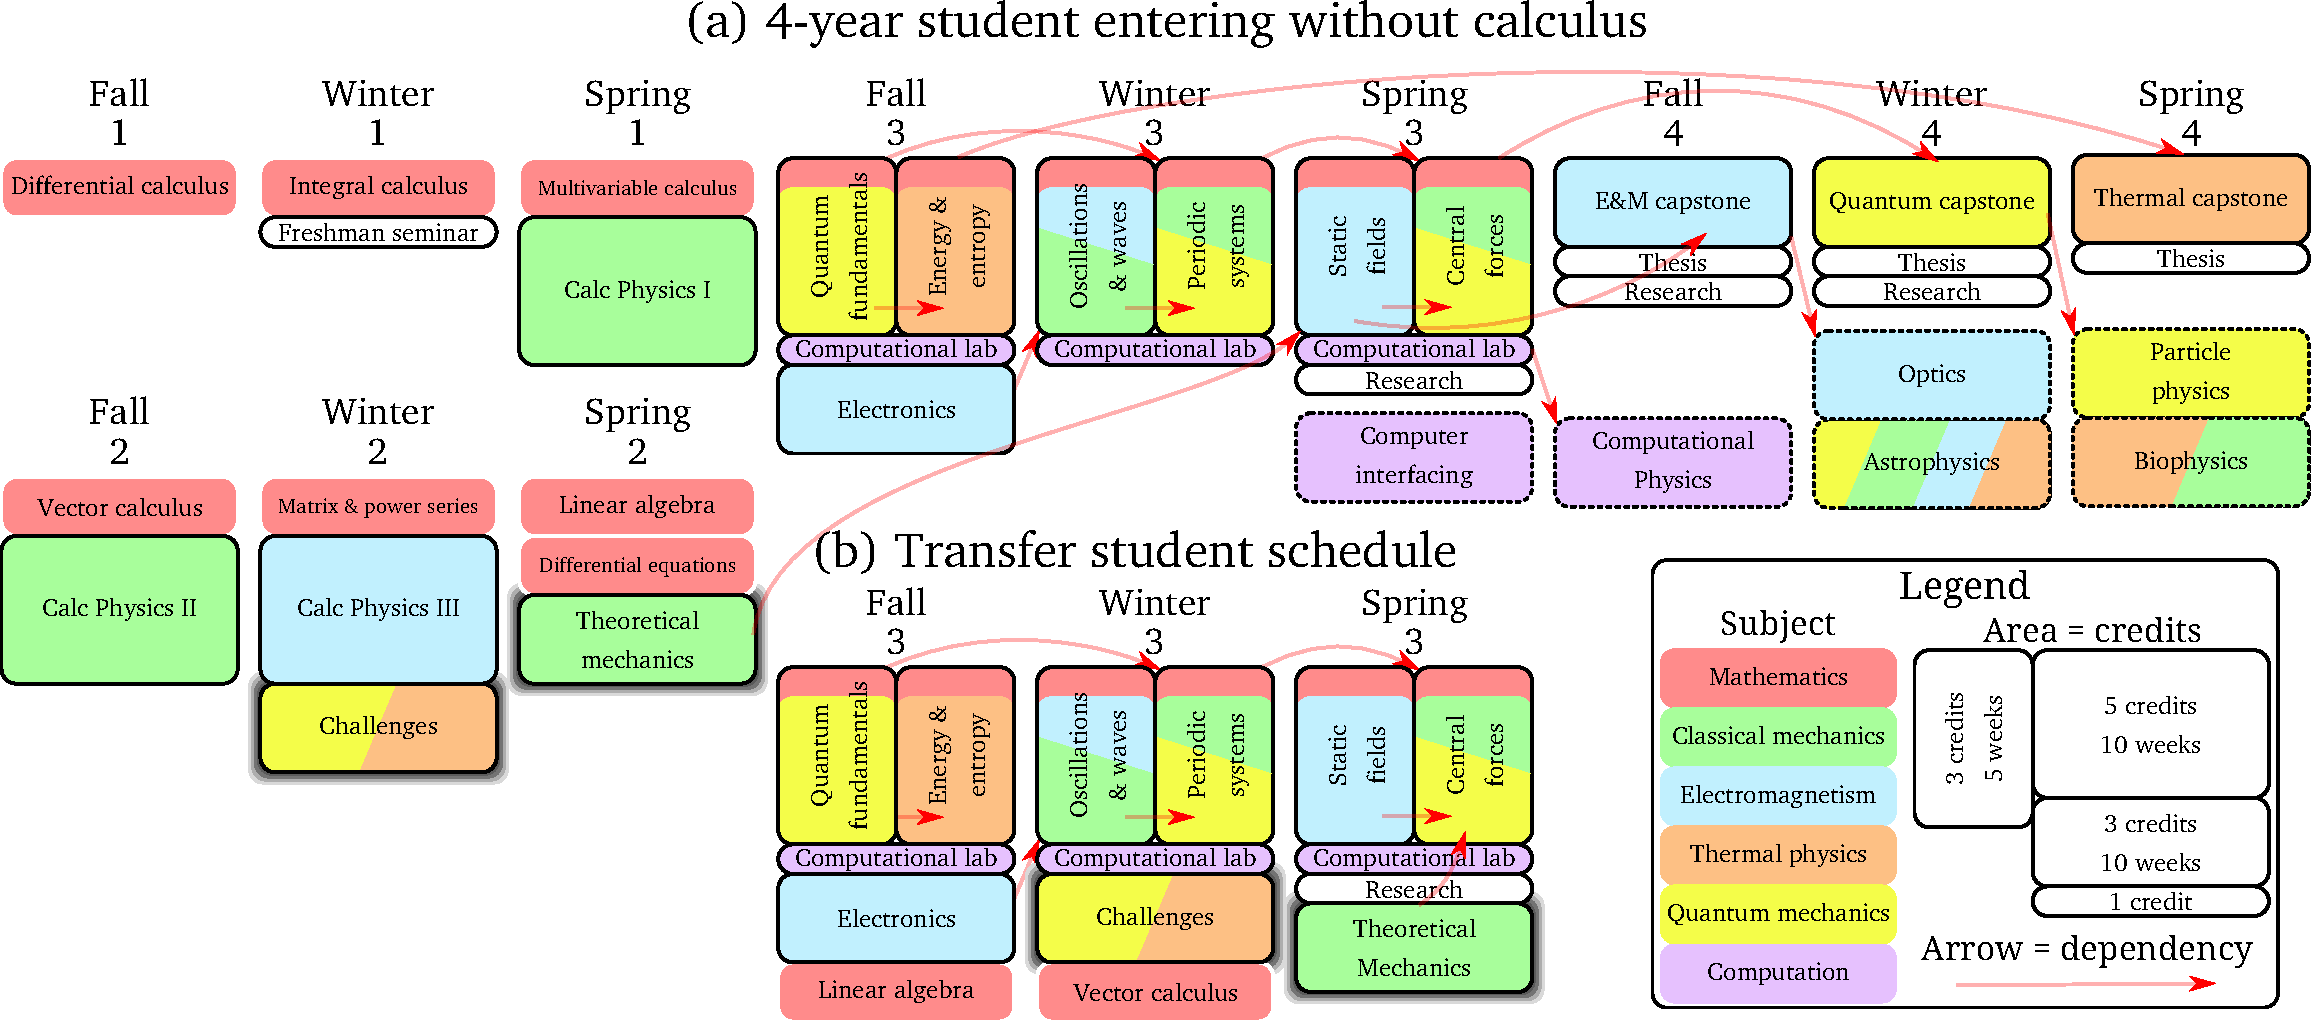
\includegraphics[width=\textwidth]{schedule}
\caption{Figure captions appear below the figure while table captions appear above the table.\label{fig1}}
\end{figure*}

% Note: Revtex puts two-column figures at the top of a page. If you really need 
% to change this, gird yourself for battle and see http://tinyurl.com/j2wnoxb.
\begin{figure*}
  %\includegraphics{figure2}
  picture here of the new curriculum
\caption{A 2-column figure. Center figure captions if they run one
  line only, and justify captions if they are multi-line.\label{fig2}}
\end{figure*}

% Formatting tweak if needed--FloatBarrier forces floats to show here, before next section
%\FloatBarrier	


\section{Conclusions}
This template was newly updated for the 2016 PERC Proceedings.  The
editors apologize if any errors exist, and encourage you to contact
them with changes and other suggestions.  

\acknowledgments{Put references below the acknowledgements (and appendixes, if any).}

% For a longer bibliography, delete the thebibliography block above, then comment in 
% these two lines to use a .bib file with BibTeX.
\bibliographystyle{apsrev}  	% supercedes the longbibliography option, so leave commented out if you want to display article titles
\bibliography{paper}  	% don't include the .bib suffix

\end{document}
